\chapter{Evaluation and results}
\label{ch:evaluation}

While previous chapters described the design, calibration, and deployment of PhenoHive at the component level, this chapter answers the main question: ``Can a student take a fresh Raspberry Pi, connect it to any Wi-Fi network, and start collecting sensor data on a shared dashboard without opening a terminal?''

\section{Test environment}
\label{sec:test-environment}

Every physical test in this chapter ran on a Raspberry Pi Zero~2\,W with DietPi~9.x, Python~3.11, and the PhenoHive service set up as in Chapter~\ref{ch:deployment}. On the server side, the UCLouvain VM ran InfluxDB~2.7 and Grafana~10.x, reached over the Tailscale overlay. Unless noted otherwise, the station communicated with the server over an ordinary residential Wi-Fi connection.

There are two limitations that apply to all tests. First is that the timing values in Table~\ref{tab:first-boot-timing} come from three to five informal manual observations. This means that they are representative of typical conditions but are not statistically rigorous measurements and that the actual durations may shift with network latency and NTP server response time. The second limitation is that the 20-station concurrent load test (Section~\ref{sec:load-test}) used one physical Raspberry Pi station and 19 software-emulated ones all running as independent Python processes on a development machine. Those emulated stations all share a single Tailscale tunnel and therefore can't reproduce independent residential network variability or hardware-level failures. This means that the test only validates server-side write capacity and auto-provisioning latency. End-to-end residential network behaviour still has to be confirmed in a live deployment.

\section{Deployment and network resilience}
\label{sec:deployment-eval}

\textbf{What was tested.} Headless first-boot onboarding: a student connects a fresh SD card, powers the Pi, and reaches live data on the shared Grafana dashboard with no terminal access.

On first boot, the \texttt{comitup} service creates a temporary hotspot. Opening \href{http://comitup.local}{http://comitup.local} after connecting to it brings up a captive portal (Figure~\ref{fig:comitup-portal}) where the student is able to pick their Wi-Fi network and type in their password \parencite{comitup-service}. The Pi will then reboot and joins the network if the credentials are correct. From there the systemd chain will then initialize the sensors and start pushing data.

\textbf{Result.} The time from power-on to live data on Grafana took under five minutes with no command-line interaction at any point. Table~\ref{tab:first-boot-timing} breaks the timing down by phase.

\begin{figure}[H]
\centering
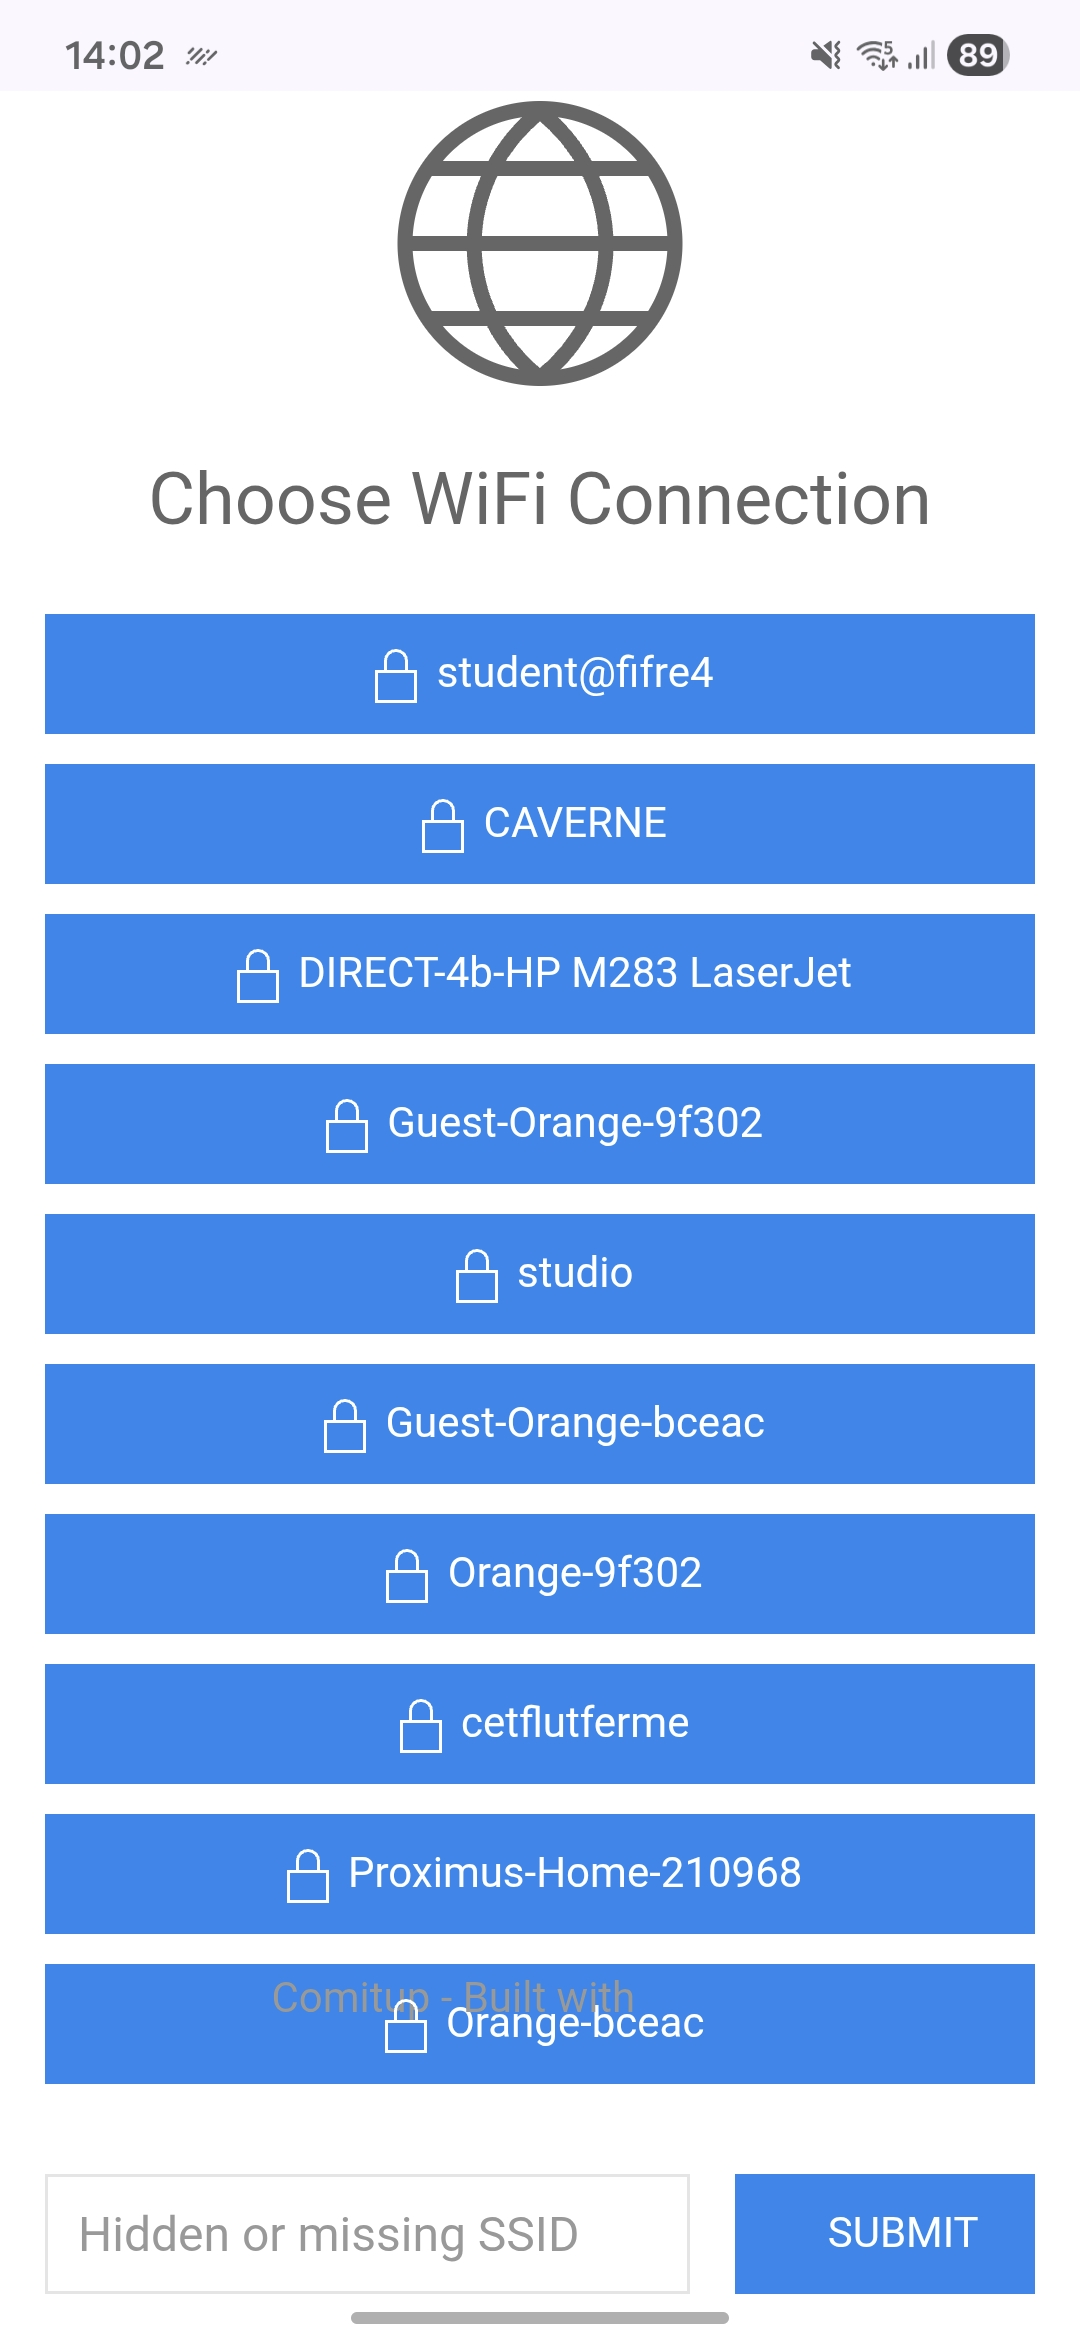
\includegraphics[width=0.4\textwidth]{Images/comitup}
\caption[The Comitup Captive Portal]{The \texttt{comitup} captive portal as seen from a smartphone. The student selects the target Wi-Fi network and enters the password. No SSH or terminal access is required.}
\label{fig:comitup-portal}
\end{figure}

\begin{table}[H]
\centering
\caption[First-Boot Setup Timing Breakdown]{Approximate timing of each phase in the first-boot setup sequence, from power-on to live data visible on the student Grafana dashboard. Values are representative estimates from testing on a Raspberry Pi Zero~2\,W; actual times depend on network speed and NTP server response latency.}
\label{tab:first-boot-timing}
\small
\renewcommand{\arraystretch}{1.25}
\begin{tabularx}{\textwidth}{|P{1.2cm}|P{2.8cm}|X|P{2.2cm}|}
\hline
\textbf{Phase} & \textbf{Milestone} & \textbf{Description} & \textbf{Approx.\ duration} \\
\hline
T0 $\to$ T1 & Power-on & Boot sequence to \texttt{comitup} hotspot broadcast & $\approx$\,45\,s \\
\hline
T1 $\to$ T2 & Portal access & Student connects to hotspot; captive portal loads in browser & $\approx$\,15\,s \\
\hline
T2 $\to$ T3 & Network join & Wi-Fi credentials submitted; Pi reboots and joins target network & $\approx$\,90\,s \\
\hline
T3 $\to$ T4 & Pre-start checks & \texttt{wait\_for\_network.sh}: internet ping and NTP synchronization confirmed & $\approx$\,30\,s \\
\hline
T4 $\to$ T5 & Sensor init & Concurrent \texttt{setup()} calls across all sensors (15\,s global timeout) & $\approx$\,15\,s \\
\hline
T5 $\to$ T6 & First write & First measurement record successfully written to InfluxDB & $\approx$\,10\,s \\
\hline
T6 $\to$ T7 & Provisioning & Auto-provisioning detects new \texttt{station\_id}; Grafana dashboard and student account created & $<$\,60\,s \\
\hline
\textbf{T0 $\to$ T7} & \textbf{Total} & \textbf{Power-on to live data on student dashboard} & $\mathbf{<}$\,\textbf{5\,min} \\
\hline
\end{tabularx}
\end{table}

\section{Runtime behaviour}
\label{sec:runtime-behaviour}

\subsection{Debug UI and on-device calibration}

\textbf{What was tested.} That the on-device web UI gives students access to live sensor readings and guided calibration without any terminal interaction.

The debug UI is a single-page web app that's hosted on port~8080 of the RPI and it has no external dependencies. Its live tab (Figure~\ref{fig:debug-ui-live}) refreshes on its own and shows temperature, humidity, weight and the 14 TCS3448 spectral channel intensities. The calibration tab (Figure~\ref{fig:debug-ui-calibrate}) walks the student through the scale calibration and the camera setup. The admins can also change settings from within this webpage instead of editing the \texttt{config.ini} file directly and see some relevant debugging information.

\textbf{Result.} Every calibration and diagnostics operation ran successfully through the browser, with no command-line interaction needed.

\begin{figure}[H]
\centering
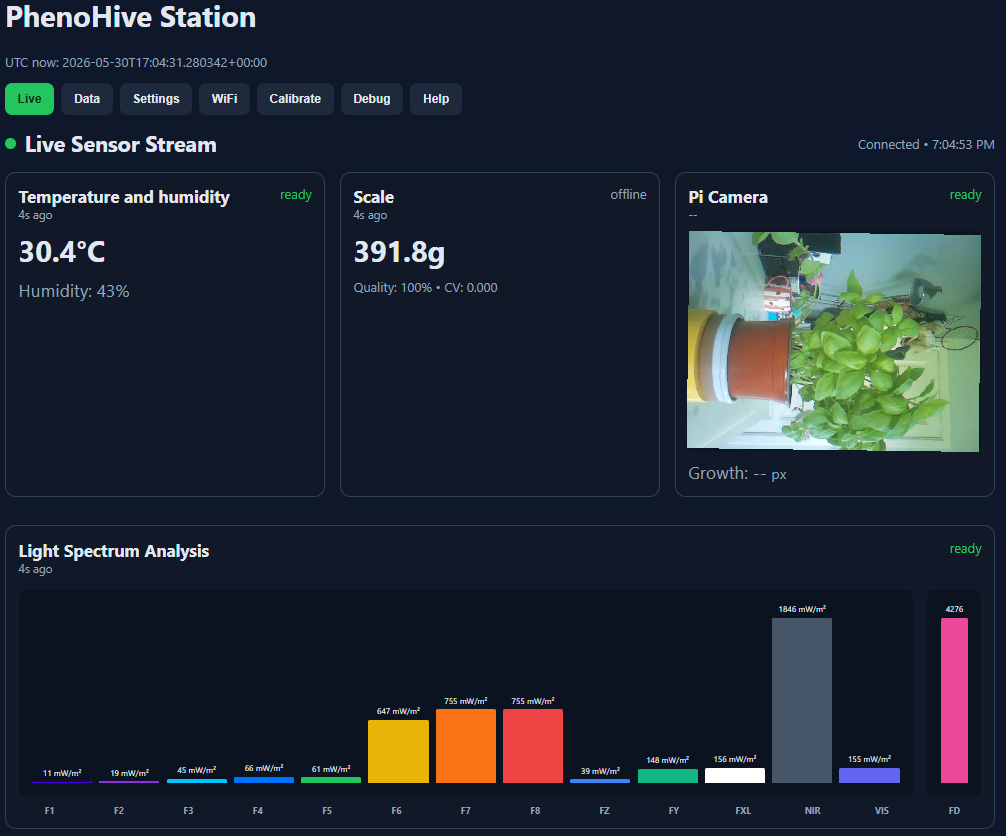
\includegraphics[width=0.85\textwidth]{Images/Debug}
\caption[Debug UI Live Sensor Tab]{The Debug UI live tab showing real-time readings from all sensors. The spectral bar chart (bottom) visualizes the live data from the 14 TCS3448 channels. The temperature, humidity and weight live values are displayed as large numeric cards. The interface refreshes every few seconds via Asynchronous JavaScript and XML (AJAX) polling.}
\label{fig:debug-ui-live}
\end{figure}

\begin{figure}[H]
\centering
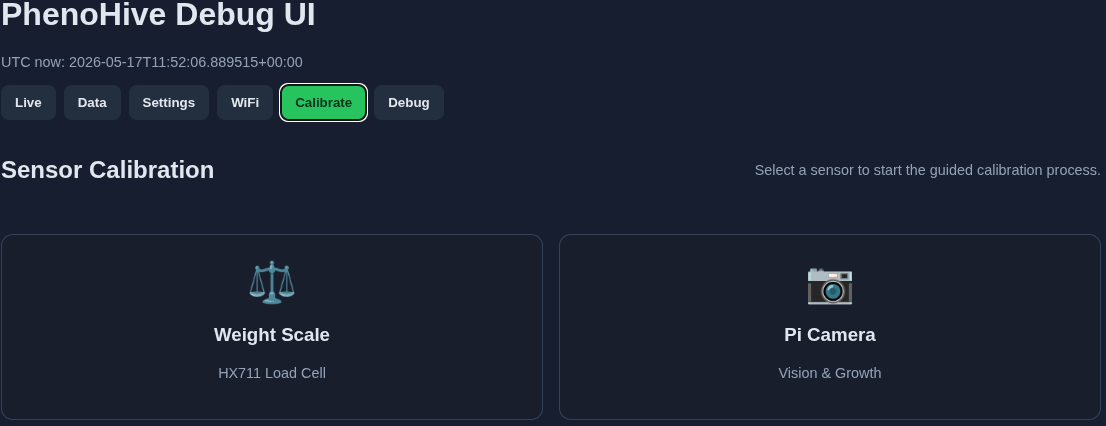
\includegraphics[width=0.85\textwidth]{Images/calibratescreen}
\caption[Debug UI Calibration Wizard]{The guided scale and camera calibration wizards in the Debug UI. Students can calibrate the scale and camera from this easy to understand interface through a guided step-by-step process where no command-line interaction is needed.}
\label{fig:debug-ui-calibrate}
\end{figure}

\subsection{Sensor data quality over a multi-day run}

\textbf{What was tested.} That the full pipeline — burst sampling, MAD outlier filtering, smoothed aggregation, and InfluxDB write — captures continuous, clean environmental data over multiple days.

Figure~\ref{fig:real-sensor-data} shows nine days of data from the physical station (2026-05-18 to 2026-05-27) across three representative channels: air temperature, relative humidity, and TCS3448 spectral channel~F6.

\textbf{Result.} All three channels recorded continuously without any gaps in the data. This demonstrates the long term stability of the platform as a whole.

\begin{figure}[H]
    \centering
    \begin{subfigure}[b]{\textwidth}
        \centering
        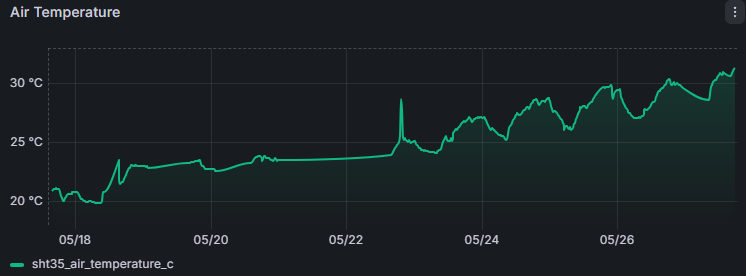
\includegraphics[width=0.92\textwidth]{Images/example_sampling_sht35_temp}
        \caption{Air temperature (\textdegree C), 2026-05-18 to 2026-05-27. A transient spike is visible around 2026-05-22; the two-stage MAD pipeline removes it before the record is persisted.}
        \label{fig:real-data-temp}
    \end{subfigure}
    \vspace{0.5em}
    \begin{subfigure}[b]{\textwidth}
        \centering
        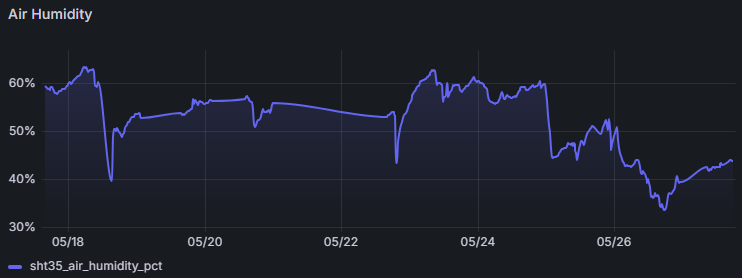
\includegraphics[width=0.92\textwidth]{Images/example_sampling_sht35_hum}
        \caption{Relative humidity (\%\,RH) which was taken during the same period. The trace is clean and continuous with no visible artefacts.}
        \label{fig:real-data-hum}
    \end{subfigure}
    \vspace{0.5em}
    \begin{subfigure}[b]{\textwidth}
        \centering
        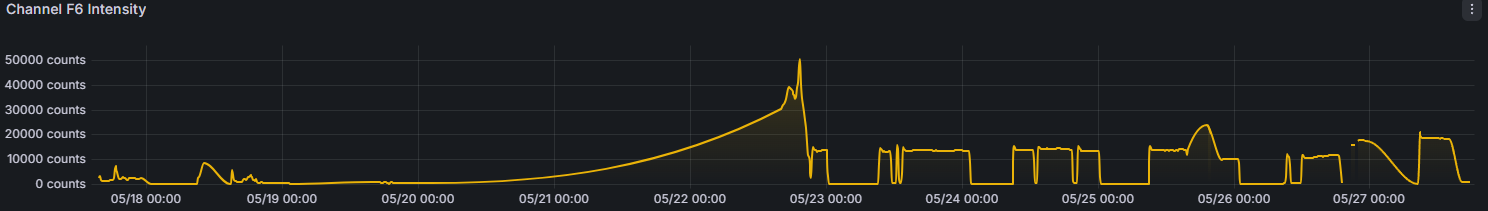
\includegraphics[width=0.92\textwidth]{Images/example_sampling_tcs3448}
        \caption{TCS3448 channel F6 intensity (counts, empirical peak $\sim$600--620\,nm). It shows a clear day and night cycle that reflects the station's lighting environment.}
        \label{fig:real-data-tcs}
    \end{subfigure}
    \caption[Nine Days of Continuous Real Sensor Data]{These are nine days of continuous sensor data from the physical PhenoHive station, as visualized on the Grafana student dashboard. The three channels that are shown here (air temperature, relative humidity, and one TCS3448 spectral channel) demonstrate the pipeline's ability to capture multi-day environmental dynamics with the temporal resolution and data quality required for plant-physiology interpretation. They also show the platform's stability long term.}
    \label{fig:real-sensor-data}
\end{figure}

\subsection{Demonstrative plant observation}
\label{sec:plant-run}

\textbf{What was tested.} That the calibrated sensor suite does indeed detect the physiological signals that the course targets when monitoring an actual potted plant. These are cumulative water loss via the pot-mass channel, atmospheric evaporative demand derived from the calibrated temperature and humidity, and light-cycle structure from the spectral channel.

A potted plant was placed on the station and monitored from 2026-05-29 to 2026-05-31 without watering. This allowed an uninterrupted trace across all channels to be made (Figure~\ref{fig:plant-run}).

The plant mass (Figure~\ref{fig:plant-run-mass}) declined linearly from 478\,g to 353\,g over 54 hours which represents a total loss of 125\,g or ($\approx$55\,g/day). Two features of this trace are notable. First is that the decline is nearly linear with no day-night acceleration. This strongly suggests that a load-cell drift under sustained load is contributing to a constant offset alongside the real water loss. The HX711 ADC is known to drift with temperature changes over hours-to-days timescales. The calibration that was carried over from \textcite{colinet2025} provides no drift correction. Second, slope changes over shorter windows (1--2 hours) remain qualitatively interpretable. A periodic re-taring protocol which is identified as future work in Section~\ref{sec:future-work} would restore quantitative multi-day accuracy.

Temperature (Figure~\ref{fig:plant-run-temp}) however remained in the 29.5--31\,°C range with a $\approx$1\,°C diurnal amplitude. This is warmer than typical indoor conditions but was due to the weather conditions at the time of recording. Relative humidity (Figure~\ref{fig:plant-run-hum}) also rose from $\sim$42\,\%\,RH to 45--46\,\%\,RH over the test cycle with a step increase overnight on May~30th and 31st which is consistent with the plant humidifying the air that surrounds the sensor. 

The TCS3448 F4 channel (Figure~\ref{fig:plant-run-tcs3448} empirical peak $\sim$480--500\,nm, cyan-green) shows a clear natural day-night light cycle. The intensity rises from near zero at night to about 600--730\,mW/m$^2$ during the afternoon. The day-to-day variation in peak intensity reflects the changing outdoor illumination instead of just some sensor artefact.

\textbf{Result.} The temperature, humidity and spectral channels functioned continuously and captured the expected physiological structure. The mass channel however revealed a drift artefact that limits absolute multi-day rate comparisons but does not affect short-term trend analysis. This is due to a calibration-maintenance issue, not an architectural one. Together the four channels demonstrate that the platform manages to capture the signals that the course requires and that the calibrated environmental data can already fully support the stomatal-response reasoning that the course expects.

\begin{figure}[H]
    \centering
    \begin{subfigure}[b]{\textwidth}
        \centering
        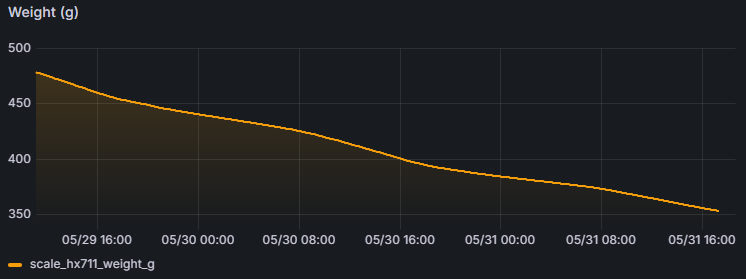
\includegraphics[width=0.92\textwidth]{Images/hx711_plant_test}
        \caption{Pot mass (g), 2026-05-29 to 2026-05-31. The nearly linear decline from 478\,g to 353\,g over about 54\,h ($\approx$55\,g/day) combines real evapotranspiration and load-cell drift. But due to the absence of day/night rate variation, it confirms that sensor drift dominates.}
        \label{fig:plant-run-mass}
    \end{subfigure}
    \vspace{0.5em}
    \begin{subfigure}[b]{\textwidth}
        \centering
        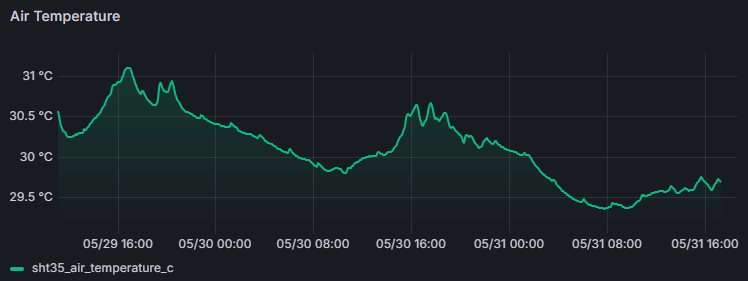
\includegraphics[width=0.92\textwidth]{Images/sht35_temp_plant}
        \caption{Air temperature (\textdegree C) during the same period. Warm and stable (29.5--31\,°C) with $\approx$1\,°C diurnal amplitude.}
        \label{fig:plant-run-temp}
    \end{subfigure}
    \vspace{0.5em}
    \begin{subfigure}[b]{\textwidth}
        \centering
        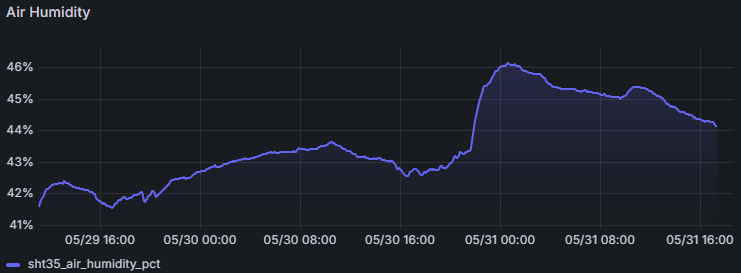
\includegraphics[width=0.92\textwidth]{Images/sht35_hum_plant}
        \caption{Relative humidity (\%\,RH) with again the same period. The rise from $\sim$42\,\% to 45--46\,\% is consistent with the plant humidifying the nearby air.}
        \label{fig:plant-run-hum}
    \end{subfigure}
    \vspace{0.5em}
    \begin{subfigure}[b]{\textwidth}
        \centering
        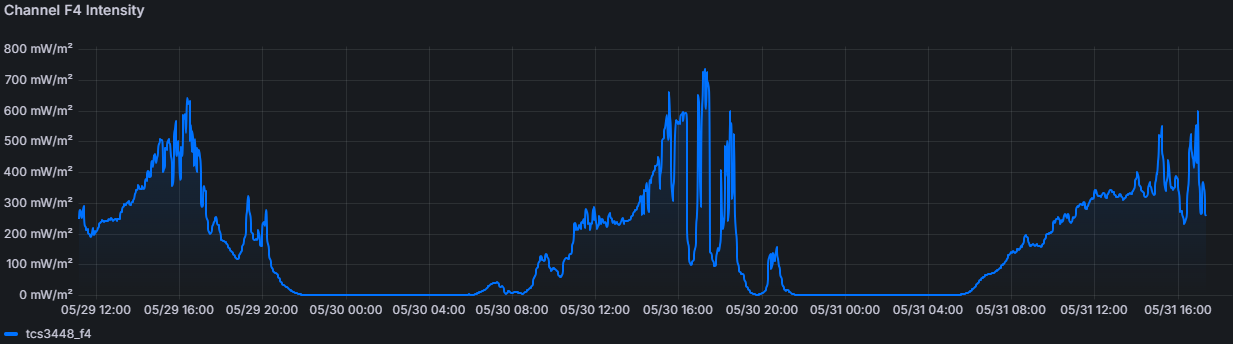
\includegraphics[width=0.92\textwidth]{Images/tcs3448_plant_test.jpg}
        \caption{TCS3448 channel~F4 (mW/m$^2$, with an empirical peak at $\sim$480--500\,nm). Natural day and night cycles are clearly visible. With a near zero value at night and 600--730\,mW/m$^2$ at afternoon peak. The day-to-day variation in peak intensity reflects changing outdoor illumination.}
        \label{fig:plant-run-tcs3448}
    \end{subfigure}
    \caption[54-Hour Plant Observation]{54-hour demonstrative plant observation (2026-05-29 to 2026-05-31).}
    \label{fig:plant-run}
\end{figure}

\subsection{Multi-station isolation and dynamic provisioning}

\textbf{What was tested.} That data is isolated per student and that reassigning a station ID triggers correct re-provisioning without data loss.

Running a physical Station~01 at the same time as a Docker-based mock Station~02 confirmed isolation at both the query and permission levels. Each student login returned only its own station's data as expected(Figures~\ref{fig:grafana-admin}--\ref{fig:grafana-student}).

To test out the dynamic provisioning path, Station~01's ID was changed to \texttt{04} through the debug UI.

\textbf{Result.} The auto-sync service built the new Grafana environment (dashboard and user account) in about two minutes. The original Station~01 dashboard retained its full history but stopped receiving new data once the ID was changed. No data loss occurred during the transition.

\begin{figure}[H]
\centering
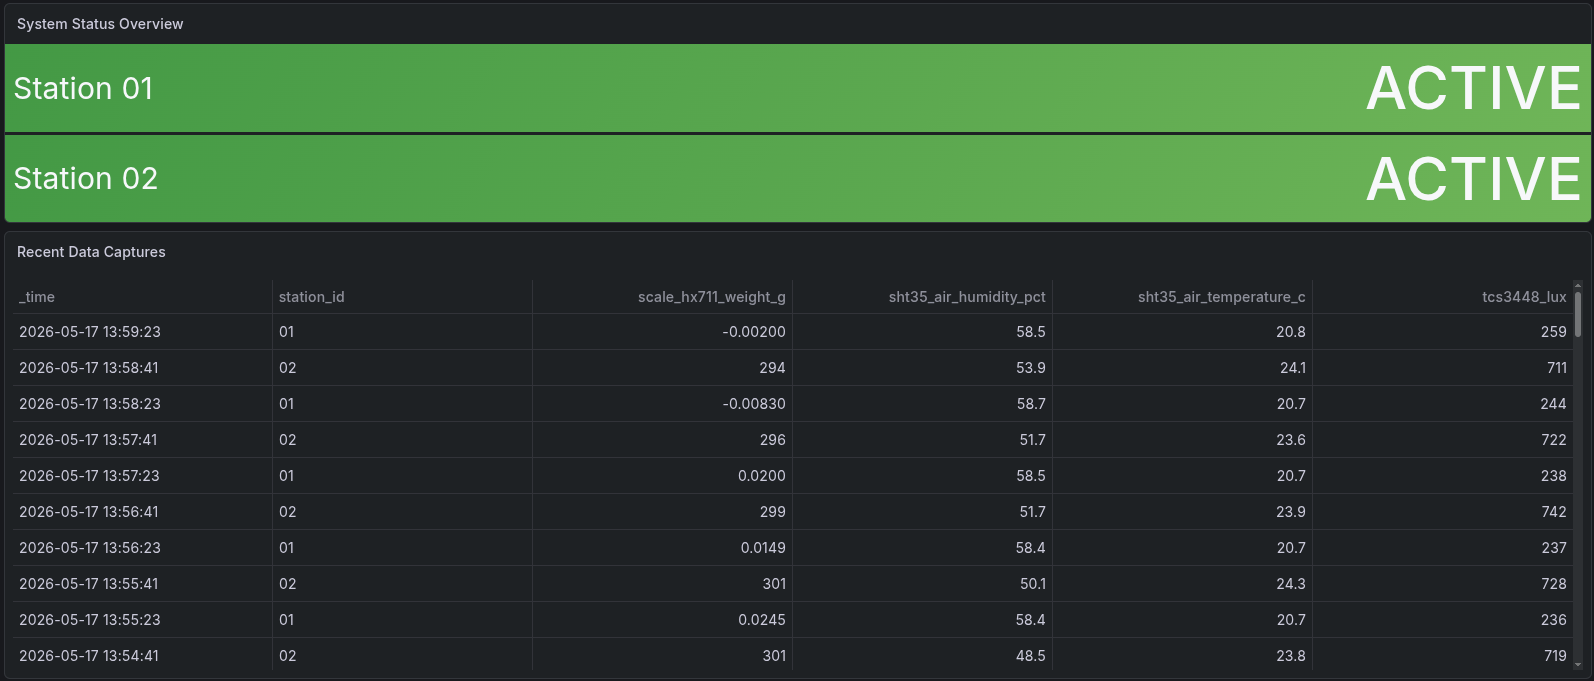
\includegraphics[width=0.85\textwidth]{Images/admingrafana}
\caption[Grafana Admin Panel]{The Grafana Admin Panel showing two active stations. Station~01 runs on physical hardware and Station~02 is a Docker-based mock. Both report the ``UP'' status with their most recent measurements visible in the unified table.}
\label{fig:grafana-admin}
\end{figure}

\begin{figure}[H]
\centering
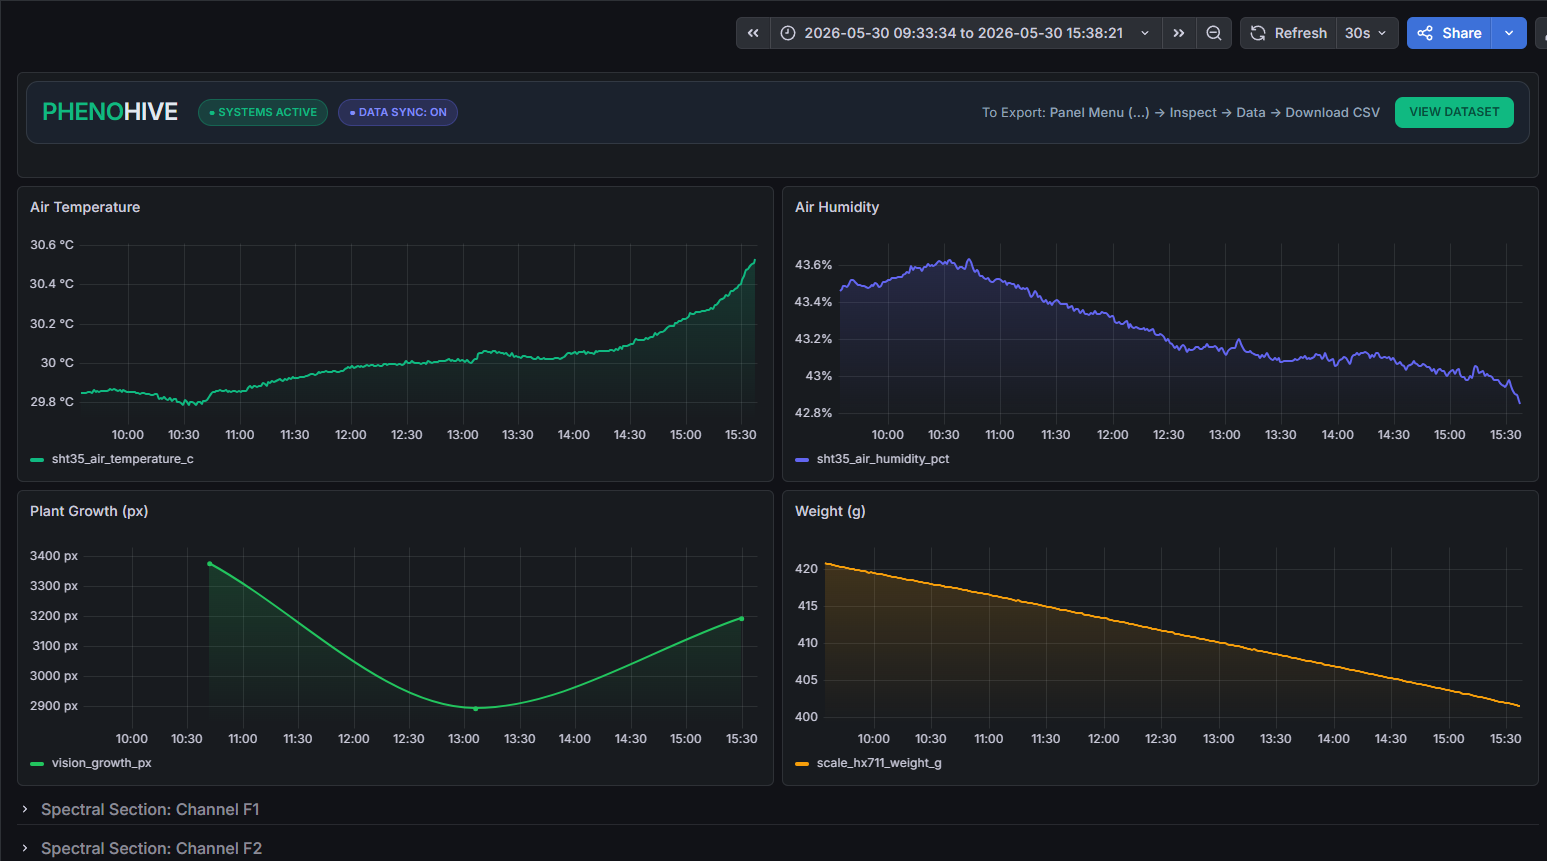
\includegraphics[width=0.85\textwidth]{Images/studentdashboard}
\caption[Student-Facing Grafana Dashboard]{The student-facing Grafana dashboard for Station~01 which shows the time-series panels for temperature, humidity, spectral irradiance and plant weight. Logging in as \texttt{student02} would displays an identical layout but with only Station~02 data, as explained to establish query-level isolation.}
\label{fig:grafana-student}
\end{figure}

\subsection{Concurrent load test}
\label{sec:load-test}

\textbf{What was tested.} Server-side write capacity and auto-provisioning latency with 20 stations writing concurrently (1~physical + 19~software-emulated).

The 19 emulated stations all ran as independent Python processes on a development machine. They were all writing through to the same Nginx proxy to the shared InfluxDB instance. The run lasted a total of 3 hours at an accelerated 30\,s/60\,s collection and publish rate to simulate real-world usage.

\textbf{Result.} Not a single station produced an offline queue file. The auto-provisioning service had all 19 dashboards up within 60--90\,s of each station's first write which confirms that the server-side write capacity and that the provisioning latency hold up at classroom level scale. As noted in Section~\ref{sec:test-environment}, the emulated stations shared a single Tailscale tunnel and could not reproduce independent residential network variability. This means that the end-to-end home-network behaviour still needs validation in a live deployment.

\section{Validation summary}
\label{sec:eval-summary}

Table~\ref{tab:eval-summary} lists all validation scenarios and their outcomes, with traceability to the original requirements.

\small
\renewcommand{\arraystretch}{1.3}
\begin{longtable}{|P{3.0cm}|p{\dimexpr\textwidth-3.0cm-2.5cm-1.8cm-8\tabcolsep-5\arrayrulewidth\relax}|P{2.5cm}|P{1.8cm}|}
\caption[System-Level Validation Test Summary]{Summary of system-level validation tests and their traceability to the original requirements. All tests were performed on physical hardware (Raspberry Pi Zero 2~W) except the 20-station load test (1 physical + 19 software-emulated).}
\label{tab:eval-summary} \\
\hline
\textbf{Test scenario} & \textbf{Expected outcome} & \textbf{Outcome} & \textbf{Req.} \\
\hline
\endfirsthead
\multicolumn{4}{l}{\small\itshape (Table~\ref{tab:eval-summary} continued from previous page)} \\[2pt]
\hline
\textbf{Test scenario} & \textbf{Expected outcome} & \textbf{Outcome} & \textbf{Req.} \\
\hline
\endhead
\hline
\endlastfoot
Headless Wi-Fi setup (fresh SD card) & Station broadcasts hotspot, accepts credentials via captive portal, begins data acquisition & Pass ($\sim$5\,min first-boot) & R3, R4 \\
\hline
Network relocation (new Wi-Fi) & Falls back to hotspot, accepts new credentials, resumes without data loss & Pass & R3 \\
\hline
48-hour server disconnection & All measurements buffered locally and replayed in order upon reconnection & Pass (no data loss observed) & R3 \\
\hline
Power-cycle reboot & Automatic reconnection and uninterrupted data resumption & Pass & R3 \\
\hline
Calibration persistence across code updates & Scale tare and factor survive deployment script execution & Pass & R3, R5 \\
\hline
Camera concurrency & Sensor polling continues at 10\,s collection interval during image capture (interval reduced from 120\,s for test visibility) & Pass & R3 \\
\hline
Sensor failure recovery & Acquisition loop continues for other sensors, and failed sensor data resumes automatically upon reconnection & Pass & R3 \\
\hline
I$^2$C bus recovery under service restart & TCS3448 and SHT35 initialize correctly after a service restart that follows an ungraceful process termination; the in-process recovery mechanism (\texttt{SensorFactory.\_run\_i2c\_recovery()}) clears the stuck bus state before each sensor setup retry & Pass & R3 \\
\hline
Persistent sensor failure watchdog & SHT35 or TCS3448 remaining in \texttt{ERROR} state for 30~min triggers an automatic service restart; both sensors recover within the first retry cycle of the new process & Pass (recovered in 1 retry cycle) & R3 \\
\hline
Station ID conflict detection & Attempting to claim an ID owned by another device is rejected & Pass & R6 \\
\hline
Multi-station data isolation & Each student login sees only their station's data & Pass & R6 \\
\hline
Dynamic ID reassignment & New Grafana environment created within 2 minutes, old dashboard retains history & Pass ($<$2\,min provisioning) & R5, R6 \\
\hline
20-station concurrent load (1 physical + 19 mock) & All write requests acknowledged, no offline queue files, all 19 dashboards auto-provisioned within 90\,s & Pass (0 queued, 19 dashboards in $<$90\,s) & R3, R6 \\
\hline
\end{longtable}
\normalsize

The validation campaign confirmed that the current implementation meets all six original requirements. Headless onboarding, multi-day network resilience, sensor-failure recovery, multi-station isolation, and concurrent 20-station operation were each demonstrated on physical hardware or a close emulation. The result that matters most in practice is the five-minute first boot: a fresh station with no prior configuration reaches live data on the shared dashboard with no command-line interaction, which is exactly the usability bar a teaching platform has to clear.
